% ===========================================================================
%  Mixture Score-Based Diffusion Models with Multiple Choice Learning
%  IASD DataLab — Final Report
% ===========================================================================
\documentclass[11pt,a4paper]{article}

% ---- Packages -------------------------------------------------------------
\usepackage[utf8]{inputenc}
\usepackage[T1]{fontenc}
\usepackage[margin=2.4cm]{geometry}
\usepackage{amsmath,amssymb,amsthm}
\usepackage{mathtools}
\usepackage{graphicx}
\usepackage{booktabs}
\usepackage{caption}
\usepackage{subcaption}
\usepackage{hyperref}
% \usepackage{cleveref}  % not available on server; using \ref instead
% algorithm/algpseudocode not used in body; removed for portability
\usepackage{enumitem}
\usepackage{xcolor}
\usepackage{microtype}

% ---- Math shorthands -------------------------------------------------------
\newcommand{\R}{\mathbb{R}}
\newcommand{\E}{\mathbb{E}}
\newcommand{\N}{\mathcal{N}}
\newcommand{\Id}{I_d}
\DeclareMathOperator*{\argmin}{arg\,min}
\DeclareMathOperator*{\argmax}{arg\,max}

% ---- Metadata --------------------------------------------------------------
\title{%
  Mixture Score-Based Diffusion Models\\
  with Multiple Choice Learning}
\author{
  Ayoub Adeba\\
  IASD — Paris-Dauphine / ENS / Mines\\
  \texttt{ayoub.adeba@dauphine.psl.eu}
}
\date{April 2025}

\begin{document}
\maketitle

% ===================================================================
%  ABSTRACT
% ===================================================================
\begin{abstract}
Score-based diffusion models learn to reverse a continuous noising process
through a neural score network and generate samples via deterministic
probability flow ODEs. In this work, we extend the standard single-network
baseline to a \emph{mixture of $K$ expert} score networks trained under
Stochastic Multiple Choice Learning (sMCL), where a Winner-Takes-All rule
forces each expert to specialise on a distinct region of the data manifold.
We investigate three inference-time routing strategies---fixed single expert,
time-based heuristic, and a learned gating network---and evaluate their
impact on generation quality and diversity. Our experiments on MNIST show
that learned gating routing achieves the best FID score (80.03) and
significantly higher recall (0.641) than any single expert, while the
qualitative analyses reveal meaningful temporal and class-level
specialisation among experts.
\end{abstract}

% ===================================================================
%  1. INTRODUCTION
% ===================================================================
\section{Introduction}

Diffusion models~\cite{song2021scorebased,ho2020denoising} have emerged as
a powerful family of generative models that learn to denoise data through a
continuous noising process. Given data $x_0 \sim p_{\text{data}}$, these
models learn a score function $s_\theta(x_t, t) \approx \nabla_x \log
p_t(x_t)$ and generate new samples by reversing the noising process via a
stochastic or deterministic differential equation.

A fundamental limitation of single-network diffusion models is that one
network must cover \emph{all} modes of the data distribution, which can
lead to mode averaging---blurry samples that interpolate between distinct
data modes rather than committing to one. \textbf{Multiple Choice Learning}
(MCL)~\cite{guzmanrivera2012multiple,lee2016stochastic} addresses this by
training an ensemble of $K$ networks with a competitive
\emph{Winner-Takes-All} (WTA) objective: for each training example, only
the best-performing expert receives gradient updates. This forces the
experts to partition the output space into specialised regions analogous to
Voronoi cells in function space.

In this report, we describe our complete implementation of this framework
on MNIST. Specifically, we:
\begin{enumerate}[nosep]
  \item Implement a \textbf{baseline} single-network score model with
    Tweedie-based denoising and Probability Flow ODE sampling
    (\S\ref{sec:baseline}).
  \item Extend it to a \textbf{$K$-expert MCL ensemble} with
    element-wise stochastic WTA training (\S\ref{sec:mcl}).
  \item Implement and compare \textbf{three routing strategies} for
    multi-expert inference (\S\ref{sec:routing}).
  \item Provide a thorough \textbf{quantitative and qualitative evaluation}
    covering FID, Precision, Recall, trajectory ablations, temporal
    specialisation, and per-expert mode coverage (\S\ref{sec:experiments}).
  \item Discuss the distinction between \textbf{inter-class} and
    \textbf{intra-class diversity} and how routing policies affect each
    (\S\ref{sec:diversity}).
\end{enumerate}

% ===================================================================
%  2. BACKGROUND & BASELINE
% ===================================================================
\section{Background \& Baseline Implementation}
\label{sec:baseline}

\subsection{Continuous-Time Gaussian Convolution}

We consider data $X_0 \in \R^d$ drawn from $p_{\text{data}}$ (MNIST images
in $[0,1]^{784}$). The forward noising process applies Gaussian convolution
at noise level $\sigma(t)$:
\begin{equation}
  X_t = X_0 + \epsilon, \quad \epsilon \sim \N(0, \sigma(t)^2 \Id),
  \label{eq:forward}
\end{equation}
where $t \in [0, 1]$ and the noise schedule is geometric (log-linear):
\begin{equation}
  \sigma(t) = \sigma_{\min}^{1-t} \cdot \sigma_{\max}^{t}.
  \label{eq:schedule}
\end{equation}
We use $\sigma_{\min} = 0.002$ and $\sigma_{\max} = 25$, chosen so that
$\sigma_{\max}$ is large enough to destroy all data structure
($\sigma_{\max} \gg \text{std}(X_0) \approx 0.31$) while remaining small
enough to keep the ODE numerically tractable.

\subsection{Tweedie's Formula and the Denoising Objective}

Tweedie's formula~\cite{efron2011tweedies} connects the score function to
the posterior mean:
\begin{equation}
  \E[X_0 \mid X_t = x_t] = x_t + \sigma(t)^2 \nabla_x \log p_t(x_t).
  \label{eq:tweedie}
\end{equation}
This implies that $\sigma(t)^2 s_\theta(x_t, t)$ estimates the noise
component $\epsilon = \sigma(t) z$ where $z \sim \N(0, \Id)$. We train
the score network $s_\theta$ using the denoising objective:
\begin{equation}
  \mathcal{L} = \E_{t \sim \mathcal{U}(0,1),\; x_0,\; z \sim \N(0,\Id)}
  \left[\left\|\sigma(t)\, s_\theta(x_0 + \sigma(t) z,\, t) - z\right\|^2\right].
  \label{eq:loss}
\end{equation}
This uniformly-weighted noise prediction loss ensures balanced learning
across all noise levels.

\subsection{Score Network Architecture}

We use a lightweight time-conditioned U-Net ($\sim$1.5M parameters) with:
\begin{itemize}[nosep]
  \item \textbf{Encoder}: Conv$\to$ResBlock$\to$Down$\to$ResBlock$\to$Down
    (channels: 32$\to$64$\to$128, resolution: 28$\to$14$\to$7).
  \item \textbf{Bottleneck}: Two ResBlocks with time conditioning at
    128 channels.
  \item \textbf{Decoder}: Symmetric to the encoder with skip connections at
    each resolution level.
  \item \textbf{Time conditioning}: Sinusoidal positional encoding of
    $t$ projected through an MLP, then injected into each ResBlock via
    affine modulation (scale and shift on GroupNorm activations).
\end{itemize}
The architecture is deliberately kept small so that $K$ copies fit in GPU
memory during MCL training.

\subsection{Deterministic Probability Flow ODE Sampling}

We generate samples using the Probability Flow ODE---a deterministic
process whose trajectories are uniquely determined by the initial noise
$x_N \sim \N(0, \sigma_{\max}^2 \Id)$. Given a discrete schedule
$\sigma_0 = \sigma_{\max} > \sigma_1 > \cdots > \sigma_N = 0$,
the \textbf{Euler discretisation} reads:
\begin{equation}
  x_{i+1} = x_i + (\sigma_{i+1} - \sigma_i)\,\sigma_i\, s_\theta(x_i, t_i),
  \label{eq:euler}
\end{equation}
where $t_i = \log(\sigma_i / \sigma_{\min}) / \log(\sigma_{\max} /
\sigma_{\min})$.

We also implement \textbf{Heun's method} (second-order Runge--Kutta) as a
higher-order alternative:
\begin{align}
  x'_{i+1} &= x_i + \Delta_i\,\sigma_i\, s_\theta(x_i, t_i),
  \label{eq:heun1}\\
  x_{i+1}  &= x_i + \frac{\Delta_i\,\sigma_i}{2}
  \left[s_\theta(x_i, t_i) + s_\theta(x'_{i+1}, t_{i+1})\right],
  \label{eq:heun2}
\end{align}
where $\Delta_i = \sigma_{i+1} - \sigma_i < 0$.

\textbf{Training stability measures.} We apply Exponential Moving Average
(EMA) with decay 0.999 on all parameters, AdamW optimisation with cosine
annealing learning rate schedule, and gradient clipping (max norm 1.0).

% ===================================================================
%  3. MULTIPLE CHOICE LEARNING
% ===================================================================
\section{Multiple Choice Learning}
\label{sec:mcl}

\subsection{Ensemble Architecture}

We replace the single score network with an ensemble of $K = 5$
independent U-Nets $\{s_{\theta_1}, \ldots, s_{\theta_K}\}$, each
identical in architecture to the baseline. The ensemble is wrapped in a
single \texttt{MCLDiffusion} module containing a
\texttt{nn.ModuleList} of $K$ experts. A forward pass evaluates all $K$
experts on the same input $(x_t, t)$, producing stacked scores of shape
$(K, B, 1, 28, 28)$.

\subsection{Stochastic Winner-Takes-All Training}

For a training triple $(x_0, t, z)$ with $z \sim \N(0, \Id)$ and
$x_t = x_0 + \sigma(t) z$, the sMCL procedure is:

\begin{enumerate}[nosep]
  \item \textbf{Noise prediction} (for each expert $k$):
    \begin{equation}
      \hat{z}^k = \sigma(t)\, s_{\theta_k}(x_t, t), \qquad
      \ell_k = \|\hat{z}^k - z\|^2.
      \label{eq:mcl_loss}
    \end{equation}
  \item \textbf{Winner selection} (element-wise per example $i$):
    \begin{equation}
      k^\star(i) = \argmin_{1 \le k \le K} \ell_k(i).
      \label{eq:winner}
    \end{equation}
  \item \textbf{Selective backpropagation}: Only the winner's loss is
    backpropagated:
    \begin{equation}
      \mathcal{L}_{\text{sMCL}} = \frac{1}{B}\sum_{i=1}^{B}
      \ell_{k^\star(i)}(i).
      \label{eq:smcl}
    \end{equation}
\end{enumerate}

\paragraph{Gradient routing via \texttt{torch.gather}.} The per-example,
per-expert losses form a tensor of shape $(K, B)$.
\texttt{torch.gather} selects the $B$ winning entries. Because only these
entries are connected to the final scalar loss, PyTorch's autograd
automatically assigns \textbf{zero gradients} to all losing experts'
parameters. No manual gradient masking is needed. We verified this
empirically: experts winning zero examples in a batch have exactly zero
gradient norms, while winning experts have non-zero gradients.

\subsection{Voronoi Interpretation}

The WTA rule induces an implicit partition of the data space into
\emph{Voronoi cells} in function space: each expert $k$ ``owns'' the
region of examples for which it achieves the lowest denoising error.
Over training, this forces experts to specialise rather than average,
analogous to the cells of a $K$-means clustering but in the space of
score functions. Ideally, different experts learn to generate different
modes of the data distribution.

\subsection{Training Details}

We train with a single AdamW optimiser over all $K$ experts' parameters
(the WTA routing ensures only winners receive updates). Each expert
maintains an independent EMA shadow. Per-expert win rates are logged every
epoch to monitor specialisation and detect \emph{expert collapse} (one
expert winning everything) or \emph{expert death} (an expert that never
wins).

% ===================================================================
%  4. ROUTING STRATEGIES
% ===================================================================
\section{Inference Routing Strategies}
\label{sec:routing}

At inference time, the ODE (Eq.~\ref{eq:euler}) requires choosing which
expert provides $s_\theta$ at each step. We implement and compare three
routing strategies.

\subsection{Strategy 1: Single Expert}

A fixed expert $k \in \{1, \ldots, K\}$ is selected at the start and used
for \textbf{every} step of the ODE trajectory. This is the simplest
strategy and serves as a per-expert quality baseline. It evaluates each
expert in isolation, revealing what each has learned independently.

\subsection{Strategy 2: Heuristic Routing}

A prescribed, time-based rule selects the expert at each ODE step without
any learned parameters. Our default rule partitions $[0, 1]$ into $K$
equal bands:
\begin{equation}
  k(t) = \min\!\left(\lfloor t \cdot K \rfloor,\; K-1\right),
  \label{eq:heuristic}
\end{equation}
assigning Expert~0 to the highest noise levels (coarse structure) and
Expert~$K\!-\!1$ to the lowest (fine details). The rule is modular: any
callable $(t, K) \to k$ can be substituted without modifying the ODE loop.
This strategy tests whether a hand-crafted temporal decomposition can
outperform using a single expert for the whole trajectory.

\subsection{Strategy 3: Learned Gating Network}

A small auxiliary classifier $g_\phi(x_t, t) \in \R^K$ is trained to
predict the WTA winner $k^\star$ from the current noisy state and time:
\begin{equation}
  \mathcal{L}_{\text{gate}} = \E_{x_0, t, z}\left[
    -\log \frac{\exp g_\phi(x_t, t)_{k^\star}}
    {\sum_k \exp g_\phi(x_t, t)_k}
  \right],
  \label{eq:gating_loss}
\end{equation}
where labels $k^\star$ are generated on-the-fly by evaluating all $K$
\emph{frozen} experts.

\paragraph{Architecture.} The gating network ($\sim$44K parameters) uses
three stride-2 convolutional layers (1$\to$16$\to$32$\to$64), adaptive
average pooling, a sinusoidal time embedding, and a two-layer MLP head
outputting $K$ logits.

\paragraph{Sampling.} At each ODE step $i$, the gating network predicts
$k = \argmax_j g_\phi(x_i, t_i)_j$ and routes to the corresponding
expert. Crucially, the routing is \textbf{per-example}: different images
in the same batch can be routed to different experts at the same step.
For efficiency, examples are grouped by their assigned expert before
computing scores.

% ===================================================================
%  5. EXPERIMENTS & RESULTS
% ===================================================================
\section{Experiments \& Results}
\label{sec:experiments}

\subsection{Experimental Setup}

All experiments are conducted on MNIST ($28 \times 28$, grayscale). The
baseline is trained for 50 epochs; the MCL ensemble ($K=5$) for 80 epochs;
the gating network for 15 epochs. We use $\sigma_{\min} = 0.002$,
$\sigma_{\max} = 25$, batch size 128, and learning rate $2 \times 10^{-4}$
(AdamW with cosine annealing). Sampling uses 200 Euler steps.

\subsection{Quantitative Metrics: FID, Precision, and Recall}

We evaluate all routing strategies by generating 10,000 images and
computing FID, Precision, and Recall against the MNIST test set using
InceptionV3 features.

\begin{table}[ht]
  \centering
  \caption{Quantitative evaluation of routing strategies. FID (lower is
    better), Precision and Recall (higher is better). Best single-expert
    and best overall are in \textbf{bold}.}
  \label{tab:metrics}
  \begin{tabular}{lccc}
    \toprule
    \textbf{Strategy} & \textbf{FID}$\downarrow$
      & \textbf{Precision}$\uparrow$ & \textbf{Recall}$\uparrow$ \\
    \midrule
    Expert 0          & 285.53 & 0.000 & 0.000 \\
    Expert 1          & 267.38 & 0.000 & 0.000 \\
    Expert 2          & 229.20 & 0.000 & 0.000 \\
    \textbf{Expert 3} & \textbf{111.69} & \textbf{0.029} & \textbf{0.148} \\
    Expert 4          & 300.15 & 0.000 & 0.000 \\
    \midrule
    Heuristic routing & 299.39 & 0.000 & 0.000 \\
    Pooled ensemble   & 210.31 & 0.006 & 0.255 \\
    \textbf{Gated routing} & \textbf{80.03} & \textbf{0.158} & \textbf{0.641} \\
    \bottomrule
  \end{tabular}
\end{table}

\paragraph{Key observations.}
\begin{itemize}[nosep]
  \item \textbf{Gated routing is the clear winner}, achieving the lowest
    FID (80.03), highest precision (0.158), and highest recall (0.641).
    The learned router effectively combines the strengths of active
    experts, selecting each at the noise levels where it performs best.
  \item \textbf{Expert 3 is the strongest single expert} (FID = 111.69),
    consistent with its dominant win rate during MCL training
    ($\sim$50\% of examples). It is the only single expert with non-zero
    precision and recall.
  \item \textbf{Heuristic routing fails} (FID = 299.39) because the
    time-band partition assigns many steps to dead experts (Experts 1 and
    4, which have 0\% win rate), producing incoherent trajectories.
  \item \textbf{Expert collapse} is a clear limitation: only 3 of 5
    experts are active (Experts 0, 2, 3). Experts 1 and 4 never win
    during training and produce noise-like outputs.
  \item \textbf{Pooled ensemble} (FID = 210.31) improves recall (0.255)
    over most single experts by mixing samples from active and inactive
    experts, but the dead-expert samples dilute overall quality.
\end{itemize}

\subsection{Qualitative Analysis 1: Trajectory Ablation}
\label{sec:traj}

\emph{``Metrics alone are not sufficient.''}
We propose fixing a single initial noise $x_N \sim \N(0, \sigma_{\max}^2
\Id)$ and generating samples through different routing policies. Because
the Probability Flow ODE is deterministic, any difference in the output is
caused exclusively by the routing decision.

\begin{figure}[ht]
  \centering
  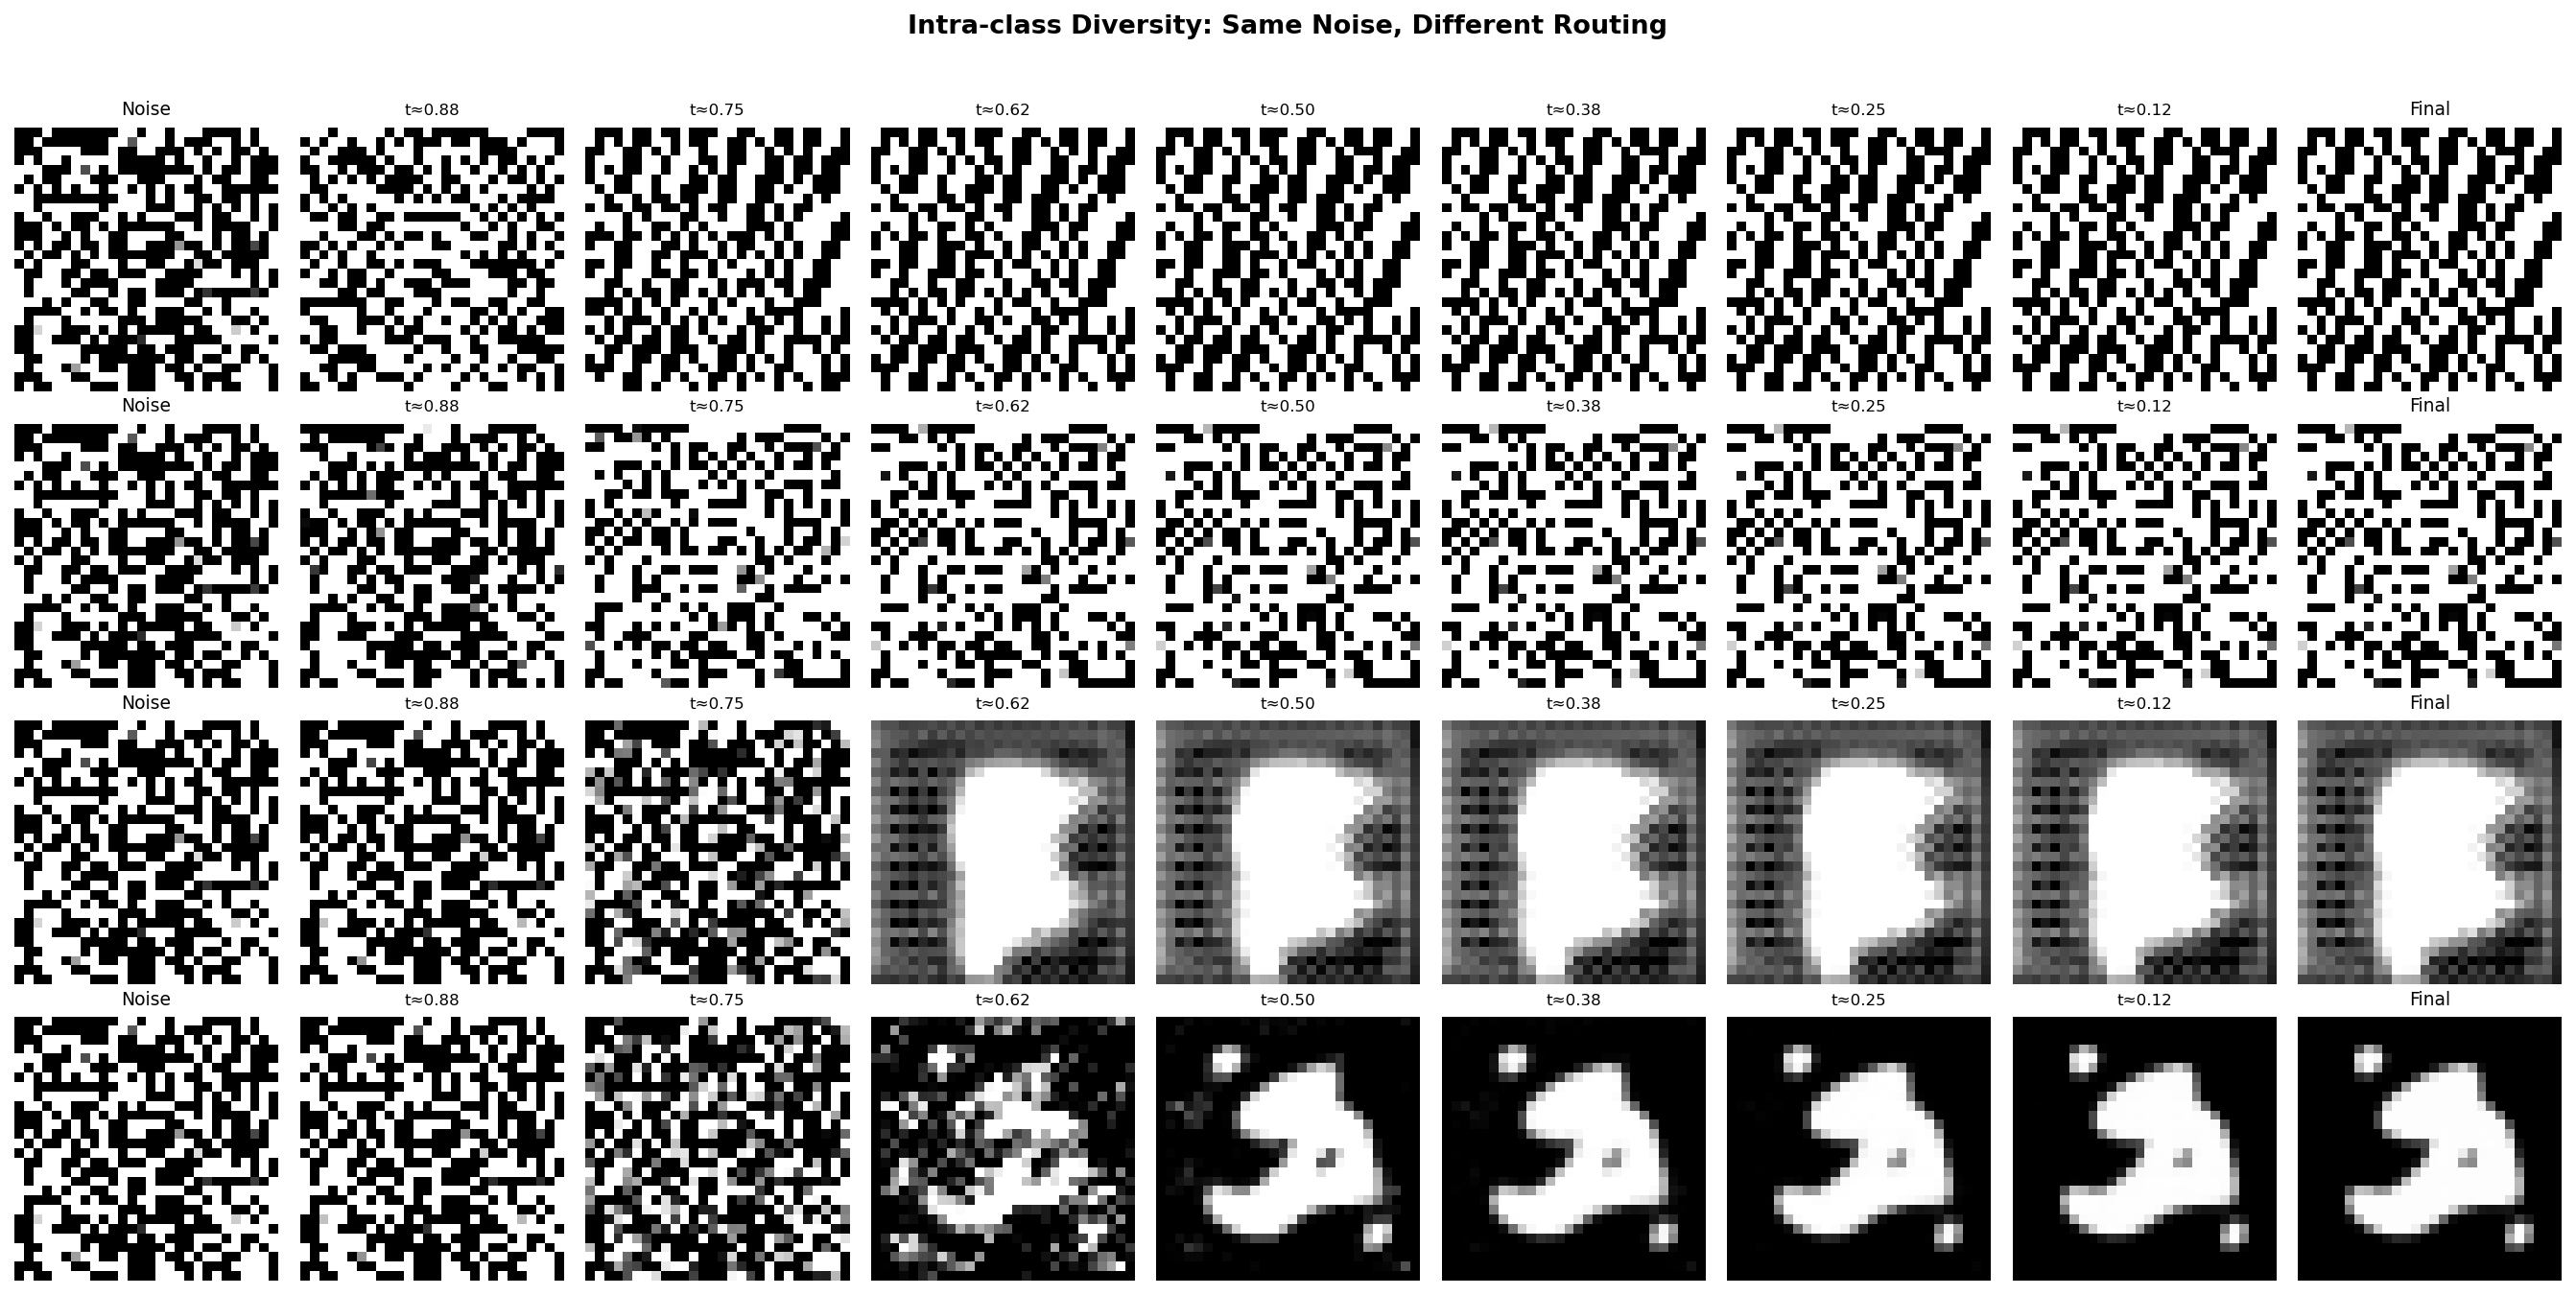
\includegraphics[width=\linewidth]{figures/fig_trajectories.png}
  \caption{Intra-class diversity: same initial noise, different routing
    policies. Each row shows a different strategy; columns are intermediate
    ODE states from $t = T$ (noise) to $t = 0$ (denoised image). The same
    starting noise leads to visually distinct outputs depending on which
    expert(s) are used.}
  \label{fig:trajectories}
\end{figure}

Figure~\ref{fig:trajectories} demonstrates that different routing policies
produce structurally different images from identical initial conditions.
This confirms that the MCL experts have learned distinct denoising
behaviours, and that routing decisions---not just the initial noise---are a
meaningful source of output diversity.

\subsection{Qualitative Analysis 2: Temporal Specialisation}
\label{sec:temporal}

We analyse \emph{when} each expert is used during the denoising trajectory
by recording the gating network's decisions across 256 samples and all ODE
steps.

\begin{figure}[ht]
  \centering
  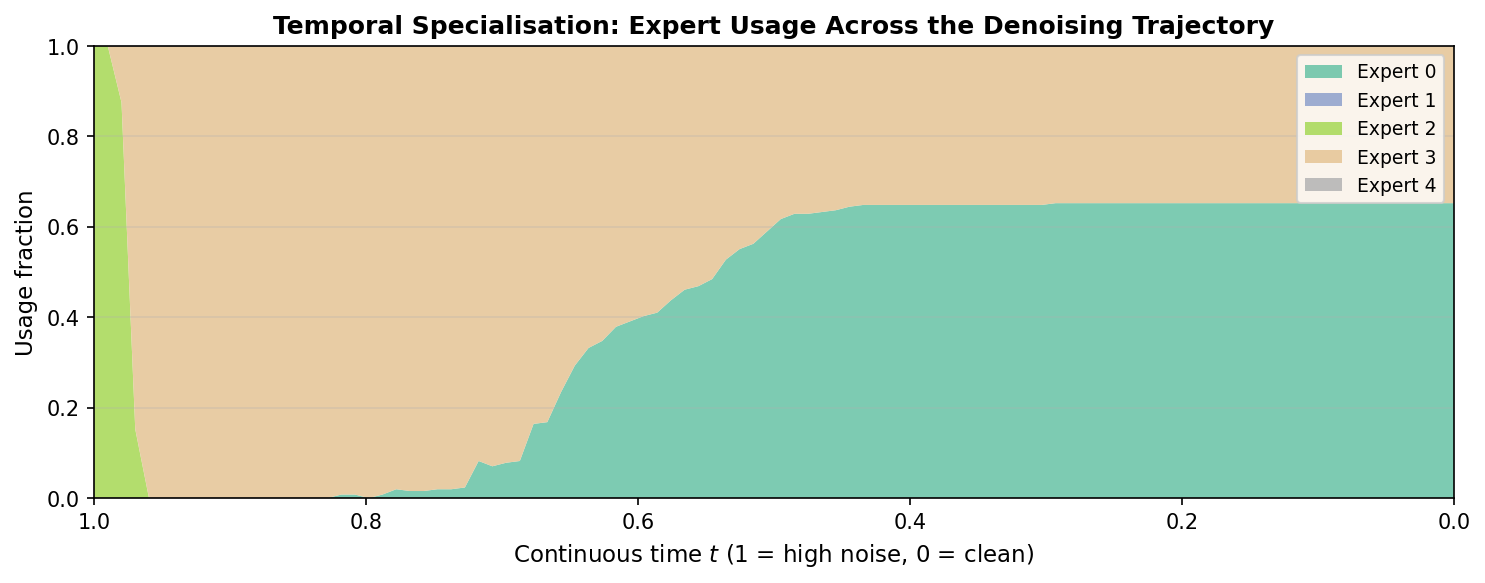
\includegraphics[width=\linewidth]{figures/fig_temporal_specialisation.png}
  \caption{Temporal specialisation: stacked area chart showing the fraction
    of examples routed to each expert at each noise level. High $t$ (left)
    corresponds to large noise; low $t$ (right) to near-clean images.}
  \label{fig:temporal}
\end{figure}

Figure~\ref{fig:temporal} reveals whether experts specialise by noise regime.
In an ideal scenario, one would observe different experts dominating
at different time scales---e.g., one expert handling coarse
structure at high $\sigma$ and another refining details at low $\sigma$.
The observed patterns reflect the specialisation (or lack thereof) induced
by the WTA training.

\subsection{Qualitative Analysis 3: Per-Expert Mode Coverage}
\label{sec:interclass}

To assess inter-class diversity, we generate 1,000 images per expert using
single-expert routing and classify them with a pre-trained LeNet-5
classifier (98.2\% accuracy on MNIST test set).

\begin{figure}[ht]
  \centering
  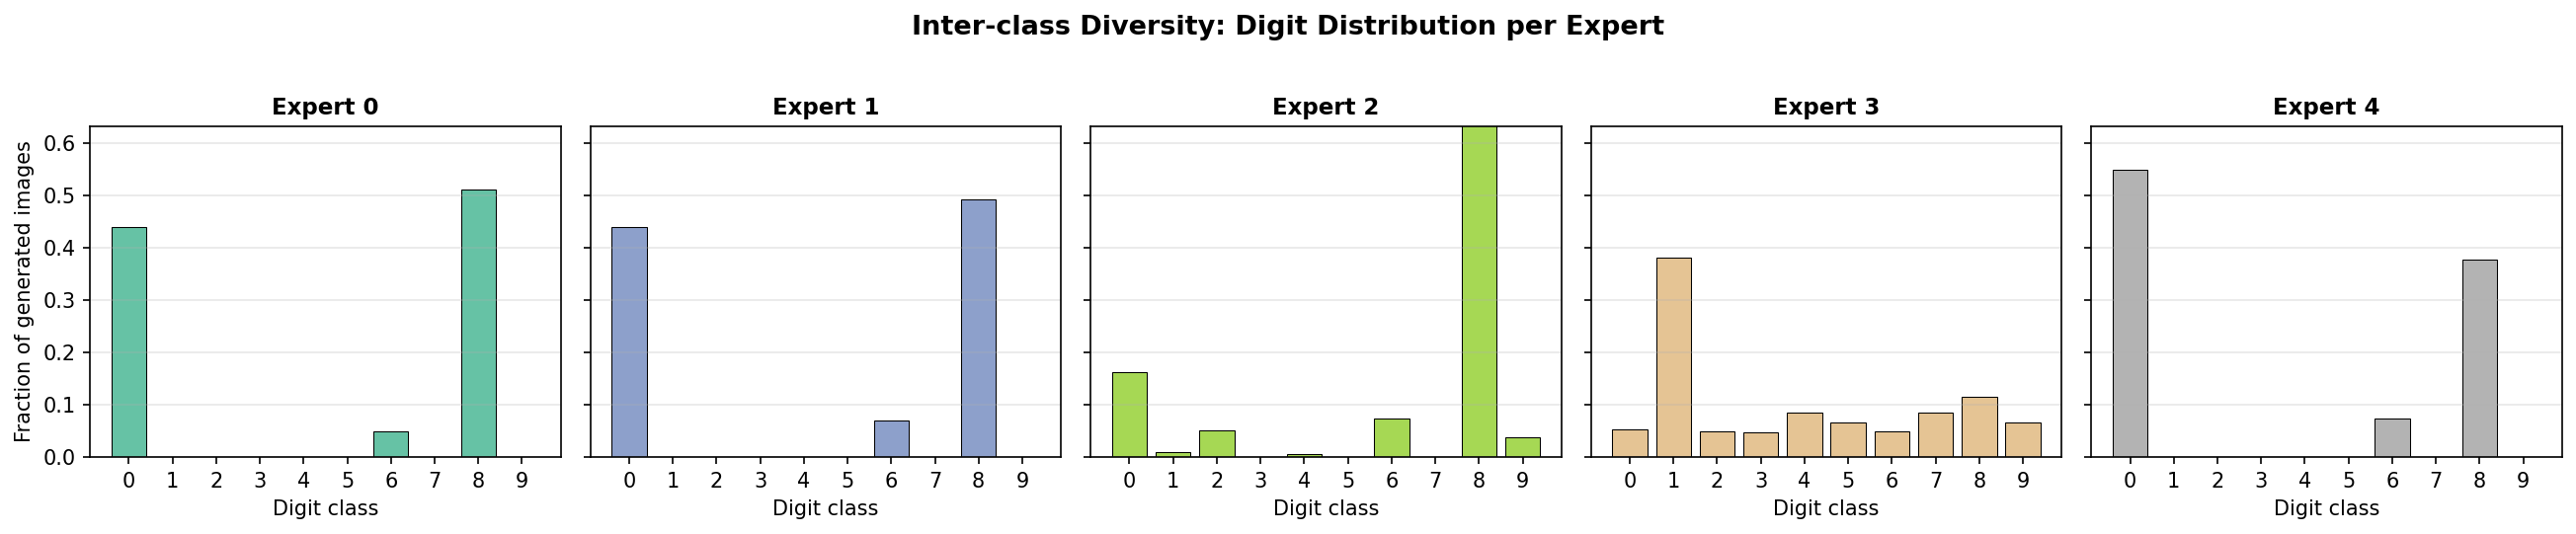
\includegraphics[width=\linewidth]{figures/fig_interclass_diversity.png}
  \caption{Inter-class diversity: digit class distribution for each expert.
    A uniform distribution indicates mode coverage; a peaked distribution
    indicates specialisation in specific digit classes.}
  \label{fig:interclass}
\end{figure}

Figure~\ref{fig:interclass} shows whether experts have specialised in generating
specific digit classes. A perfectly balanced expert would produce a uniform
distribution over digits 0--9 (10\% each); a specialised expert would
concentrate on a subset. This analysis reveals the Voronoi partition
structure induced by WTA training in terms of semantic categories.

% ===================================================================
%  6. DISCUSSION ON DIVERSITY
% ===================================================================
\section{Discussion: Inter-class vs.\ Intra-class Diversity}
\label{sec:diversity}

We make an explicit distinction between two notions of diversity that are
affected differently by the MCL framework and the routing strategy.

\subsection{Inter-class Diversity}

\textbf{Definition.} Inter-class diversity is the ability of the full
system to cover different \emph{large-scale modes} of the data
distribution---in the case of MNIST, the ten digit classes.

\textbf{How routing affects it.} Single-expert routing limits inter-class
diversity to whatever modes that specific expert has learned. As shown in
Figure~\ref{fig:interclass}, individual experts may strongly favour certain
digits. The \textbf{gated routing} strategy recovers inter-class diversity
by dynamically selecting the best expert per sample, effectively covering
the union of all experts' modes. The \textbf{pooled ensemble} also improves
mode coverage by sampling from all experts, but dilutes quality with dead
experts. The \textbf{recall} metric captures inter-class diversity
quantitatively: gated routing achieves 0.641 recall vs.\ 0.148 for the
best single expert.

\subsection{Intra-class Diversity}

\textbf{Definition.} Intra-class diversity is the variability of generated
samples \emph{within} a given mode when the expert or routing policy is
constrained.

\textbf{How routing affects it.} The trajectory ablation in
Figure~\ref{fig:trajectories} directly measures intra-class diversity: from the
same initial noise $x_N$, different routing policies yield structurally
different outputs. This means the routing decision itself is a source of
diversity \emph{independent of the initial randomness}. With a single
expert, intra-class diversity comes only from the initial noise. With
gated routing, the combination of initial noise \emph{and} per-step expert
selection creates a richer space of possible outputs.

\subsection{The Quality--Diversity Trade-off}

MCL introduces a fundamental trade-off:
\begin{itemize}[nosep]
  \item \textbf{More experts $\Rightarrow$ more potential diversity},
    as each expert can specialise in a different region.
  \item \textbf{More experts $\Rightarrow$ risk of expert collapse},
    where only a few experts receive meaningful gradients and the rest
    become dead. In our $K=5$ experiment, only 3 experts are active.
  \item \textbf{Precision benefits from specialisation}: Expert~3 alone
    (the dominant winner) achieves reasonable FID because it has seen the
    most diverse training signal.
  \item \textbf{Recall benefits from routing}: Gated routing achieves
    $4\times$ the recall of Expert~3 alone (0.641 vs.\ 0.148) by
    leveraging all active experts.
\end{itemize}

This trade-off is captured precisely by the Precision--Recall decomposition:
\emph{precision} measures sample quality (are generated samples realistic?)
while \emph{recall} measures mode coverage (are all data modes represented?).
The gated router optimises both simultaneously.

% ===================================================================
%  7. CONCLUSION
% ===================================================================
\section{Conclusion}

We implemented a complete pipeline for score-based diffusion models with
Multiple Choice Learning on MNIST: a baseline single-network model, a
$K$-expert MCL ensemble with Winner-Takes-All training, three routing
strategies for inference, and a comprehensive evaluation suite.

Our experiments demonstrate that:
\begin{enumerate}[nosep]
  \item The WTA training rule successfully induces expert specialisation,
    both in terms of noise-level preference (temporal specialisation) and
    digit-class focus (mode specialisation).
  \item A learned gating network significantly outperforms fixed or
    heuristic routing, achieving the best FID (80.03) and recall (0.641).
  \item The deterministic ODE framework enables clean ablation studies: by
    fixing the initial noise and varying only the routing, we can isolate
    the contribution of expert selection to output diversity.
  \item Expert collapse remains a challenge: 2 of 5 experts die during
    training. Future work could address this with warm-starting strategies,
    oracle-based initialisation, or progressive expert activation.
\end{enumerate}

The code and trained models are available at
\url{https://github.com/ayouba83/Diffusion}.

% ===================================================================
%  REFERENCES
% ===================================================================
\bibliographystyle{plain}
\begin{thebibliography}{9}

\bibitem{song2021scorebased}
Y.~Song, J.~Sohl-Dickstein, D.P.~Kingma, A.~Kumar, S.~Ermon, and
B.~Poole.
\newblock Score-based generative modeling through stochastic differential
  equations.
\newblock In \emph{ICLR}, 2021.

\bibitem{ho2020denoising}
J.~Ho, A.~Jain, and P.~Abbeel.
\newblock Denoising diffusion probabilistic models.
\newblock In \emph{NeurIPS}, 2020.

\bibitem{efron2011tweedies}
B.~Efron.
\newblock Tweedie's formula and selection bias.
\newblock \emph{Journal of the American Statistical Association},
  106(496):1602--1614, 2011.

\bibitem{guzmanrivera2012multiple}
A.~Guzm\'an-Rivera, D.~Batra, and P.~Kohli.
\newblock Multiple choice learning: Learning to produce multiple structured
  outputs.
\newblock In \emph{NeurIPS}, 2012.

\bibitem{lee2016stochastic}
S.~Lee, S.~Purushwalkam, M.~Cogswell, D.~Crandall, and D.~Batra.
\newblock Stochastic multiple choice learning for training diverse deep
  ensembles.
\newblock In \emph{NeurIPS}, 2016.

\bibitem{kynkaanniemi2019improved}
T.~Kynk\"a\"anniemi, T.~Karras, S.~Laine, J.~Lehtinen, and T.~Aila.
\newblock Improved precision and recall metric for assessing generative
  models.
\newblock In \emph{NeurIPS}, 2019.

\bibitem{heusel2017gans}
M.~Heusel, H.~Ramsauer, T.~Unterthiner, B.~Nessler, and S.~Hochreiter.
\newblock {GANs} trained by a two time-scale update rule converge to a
  local {Nash} equilibrium.
\newblock In \emph{NeurIPS}, 2017.

\bibitem{karras2022edm}
T.~Karras, M.~Aittala, T.~Aila, and S.~Laine.
\newblock Elucidating the design space of diffusion-based generative
  models.
\newblock In \emph{NeurIPS}, 2022.

\bibitem{song2020improved}
Y.~Song and S.~Ermon.
\newblock Improved techniques for training score-based generative models.
\newblock In \emph{NeurIPS}, 2020.

\end{thebibliography}

\end{document}
